\begin{figure}
  \center
  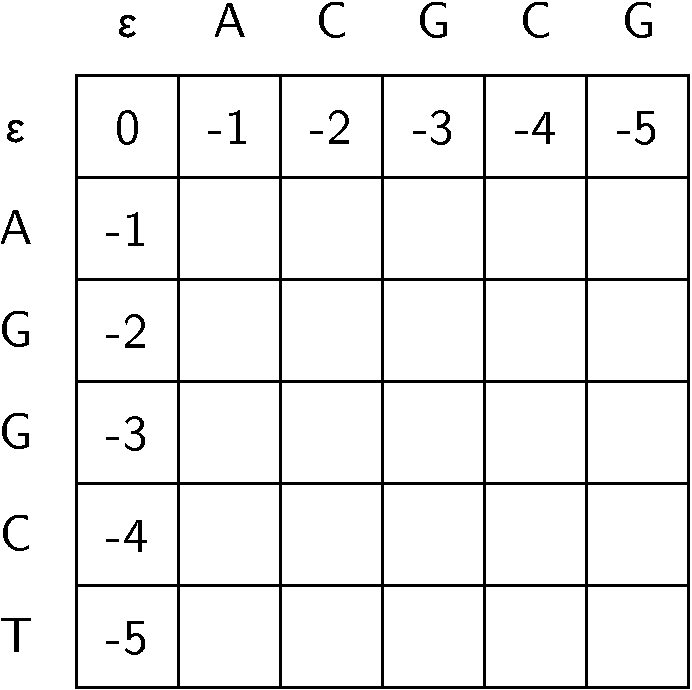
\includegraphics[width=0.3\textwidth]{fig/fig3.pdf}
  \caption{An initialized Needleman-Wunsch algorithm instance, for the input strings: \texttt{ACGCG} and \texttt{AGGCT}, with an indel score of -1.}
  \label{fig3}
\end{figure}
The algorithm works by first initiating the matrix with the south-western corner being initiatingitialized to $0$, and the wester and eastern edges being initiated, with their value being their distance from the corner, times the score for an insertion/deletion, an indel. In this report we will use the following scores:
\begin{center}
  \begin{tabular}{lc}
    Indel: & -1\\
    Mismatch: & 0\\
    Match: & 1
  \end{tabular}
\end{center}
Which results in the initialized matrix, as can be seen for an example in Figure \ref{fig3}. This is then filled out row by row, from the top down, left to right, where each value is calculated as follows:
$$
  v_{ij} =
  \begin{cases}
    \mbox{max}(v_{i-1,j-1} + \mbox{ Match, } v_{i-1,j} + \mbox{ Indel, } v_{i,j-1} + \mbox{ Indel}) & \text{if } x_i = y_i \\
    \mbox{max}(v_{i-1,j-1} + \mbox{ Misatch, } v_{i-1,j} + \mbox{ Indel, } v_{i,j-1} + \mbox{ Indel}) & \text{otherwise} %
  \end{cases}
$$
Using these rules we can populate the matrix in Figure \ref{fig3}, which results in the output matrix which is shown in Figure \ref{fig4}.
\begin{figure}[H]
  \center
  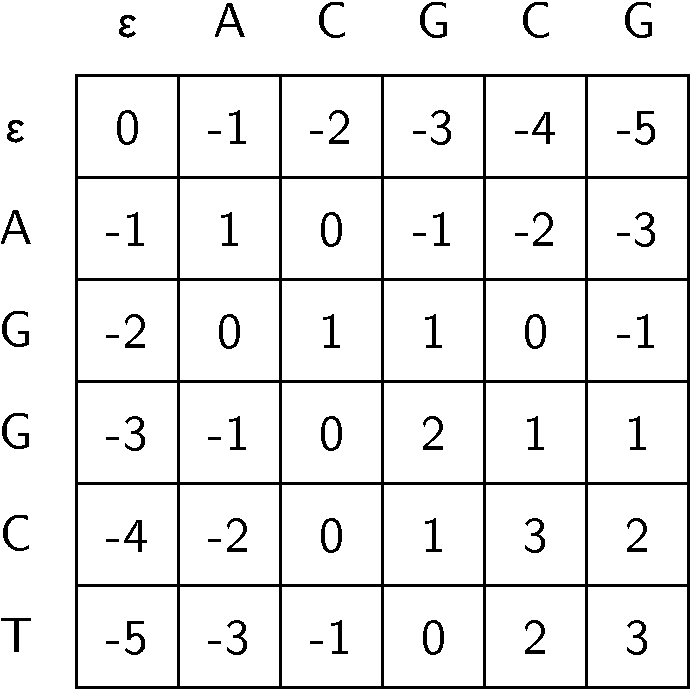
\includegraphics[width=0.3\textwidth]{fig/fig4.pdf}
  \caption{The filled out matrix corresponding to the input matrix shown in Figure \ref{fig3}.}
  \label{fig4}
\end{figure}
From the bottom right corner, the alignment score can then be read, the original algorithm will also output the entire result matrix, but the parallel version implemented will only return the alignment score.
